\documentclass{beamer}

\usepackage{pgfgantt}
\usepackage{tikz}
\usepackage{graphicx}
\usepackage{caption}
\usepackage{listings}
\usepackage{xcolor}
\usepackage{bold-extra}
\usepackage{gospel}
\usepackage{booktabs}

%\usetheme{Madrid}

\usetheme{Pittsburgh}
\usecolortheme{beaver}

\newenvironment{changemargin}[2]{%
  \begin{list}{}{%
    \setlength{\topsep}{0pt}%
    \setlength{\leftmargin}{#1}%
    \setlength{\rightmargin}{#2}%
    \setlength{\listparindent}{\parindent}%
    \setlength{\itemindent}{\parindent}%
    \setlength{\parsep}{\parskip}%
  }%
\item[]}{\end{list}}


\newcommand{\quotemarks}[1]{``#1''}
\newcommand{\bb}{\bigskip\bigskip}

\DeclareCaptionFormat{listing}{\hfill#3}
\setbeamertemplate{navigation symbols}{}

\definecolor{theblue}{rgb}{0,0,0.797}
\let\emph\alert

\AtBeginSection[]
{
    \begin{frame}[plain]{}
        \begin{center}
            {\large\emph{\insertsection}}\\
            ~\hfill\hrulefill\hfill~
        \end{center}
    \end{frame}
    \addtocounter{framenumber}{-1}
}

\makeatletter
\setbeamertemplate{footline}
{
    \leavevmode%
    \hbox{%
    \begin{beamercolorbox}[wd=.25\paperwidth,ht=2.25ex,dp=1ex,center]{author in head/foot}%
        \usebeamerfont{author in head/foot}Python Journey %\insertsection
    \end{beamercolorbox}%
    \begin{beamercolorbox}[wd=.5\paperwidth,ht=2.25ex,dp=1ex,center]{title in head/foot}%
        \usebeamerfont{title in head/foot}\insertauthor
    \end{beamercolorbox}%
    %\begin{beamercolorbox}[wd=.125\paperwidth,ht=2.25ex,dp=1ex,center]{date in head/foot}%
    %    \usebeamerfont{date in head/foot}ICE-E
    %\end{beamercolorbox}% 
    \begin{beamercolorbox}[wd=.25\paperwidth,ht=2.25ex,dp=1ex,right]{date in head/foot}%
        \insertframenumber{} / \inserttotalframenumber\hspace*{4ex} 
    \end{beamercolorbox}}%
    \vskip0pt%
}
\makeatother

%Information to be included in the title page:
\title{Introduction to Python}
\subtitle{Python Journey}
\author{Pedro Gasparinho}
%\institute{NOVA School of Science and Technology}
\date{\today}

%\titlegraphic{
%
\includegraphics[width=6cm]{../Images/en_di_rgb_positivo_h.png}
%}

%\usepackage[
%    backend=biber,
%    giveninits=true,
%    backref=true,
%    backrefstyle=three,
%    urldate=iso, 
%    date=iso,
%    seconds=true
%]{biblatex}
%\addbibresource{bibliography.bib}

\begin{document}
\captionsetup[lstlisting]{format=listing,singlelinecheck=false, margin=0pt,
  font={sf,it},labelsep=space,labelfont=bf,belowskip=-1pt}
\captionsetup{justification=centering, labelformat=simple}

\frame[plain]{\titlepage}
\addtocounter{framenumber}{-1}

%%%%%%%%%%%%%%%%%%%%%%%%%%%%%%%%%%%%%%%%%%%%%%%%%%%%%%%%%%%%%%%%%%%%%%%%%%%%%%%
%%%%% Introduction %%%%%%%%%%%%%%%%%%%%%%%%%%%%%%%%%%%%%%%%%%%%%%%%%%%%%%%%%%%%
%%%%%%%%%%%%%%%%%%%%%%%%%%%%%%%%%%%%%%%%%%%%%%%%%%%%%%%%%%%%%%%%%%%%%%%%%%%%%%%

\section*{Introduction}
%\begin{frame}
%    \frametitle{Motivation}
%    \onslide<1->{\textit{``Everybody should learn to program a computer, because it teaches you how to think.''} \\
%    \hfill {\color{theblue}{Steve Jobs, co-founder of Apple}}
%    \bb}
%    \onslide<2->{\textit{``Artificial intelligence is the science of making machines do things that would require intelligence if done by humans.''} \\
%    \hfill {\color{theblue}{John McCarthy, computer scientist}}
%    \bb}
    %\onslide<3->{\textit{``It's going to be interesting to see how society deals with artificial intelligence, but it will definitely be cool.''} \\
    %\hfill {\color{theblue}{Jeff Hawkins, computer scientist}}
    %\bb}
%    \onslide<3->{\textit{``If debugging is the process of removing software bugs, then programming must be the process of putting them in.''} \\
%    \hfill {\color{theblue}{Edsger Dijkstra, computer scientist}}
%    \bb}
%\end{frame}

%%%%%%%%%%%%%%%%%%%%%%%%%%%%%%%%%%%%%%%%%%%%%%%%%%%%%%%%%%%%%%%%%%%%%%%%%%%%%%%%%%%%%%%%%%%%%%%%%%%%%%%%%%%%%%%%%%%%%%%%%%%%%%%%%%%%%%
%%%%% Examples %%%%%%%%%%%%%%%%%%%%%%%%%%%%%%%%%%%%%%%%%%%%%%%%%%%%%%%%%%%%%%%%%%%%%%%%%%%%%%%%%%%%%%%%%%%%%%%%%%%%%%%%%%%%%%%%%%%%%%%
%%%%%%%%%%%%%%%%%%%%%%%%%%%%%%%%%%%%%%%%%%%%%%%%%%%%%%%%%%%%%%%%%%%%%%%%%%%%%%%%%%%%%%%%%%%%%%%%%%%%%%%%%%%%%%%%%%%%%%%%%%%%%%%%%%%%%%

\begin{frame}[containsverbatim]
    \frametitle{First Program}
    \begin{pythonlst}
        print('Hello World!')
    \end{pythonlst}
    \bb
    \begin{itemize}
        \item \textit{print} - Function
        \item \textit{'Hello World!'} - Value of type string
    \end{itemize}
\end{frame}

\begin{frame}
    \frametitle{Number Sets}
    \begin{minipage}[c]{0.48\linewidth}
        \centering
        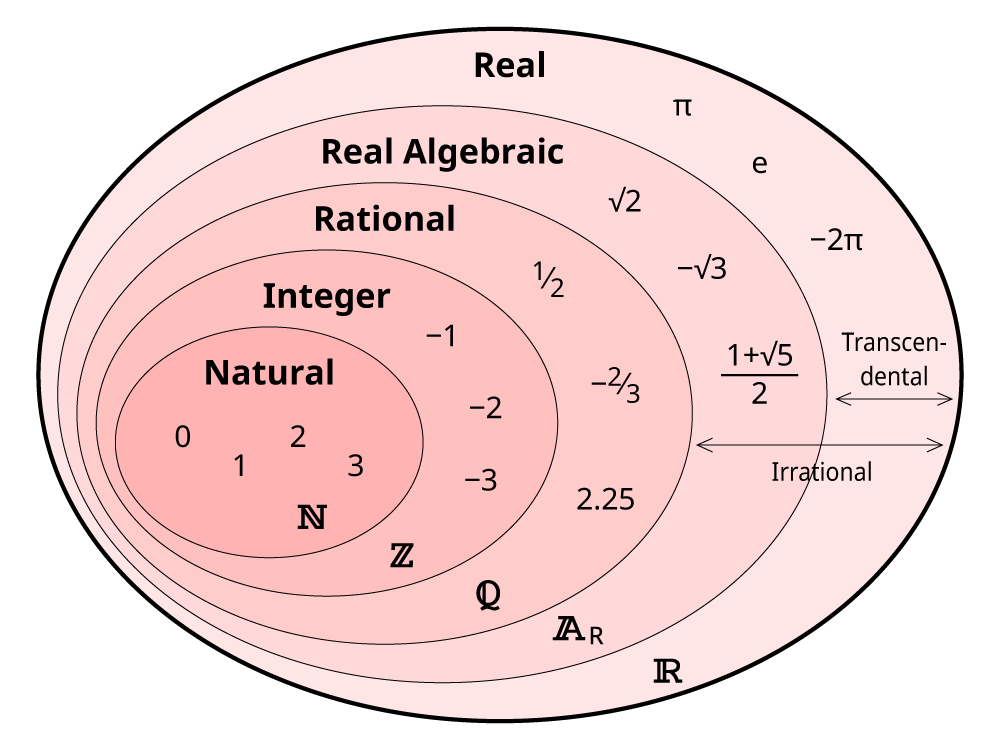
\includegraphics[width=\textwidth]{../Images/RealSet_w1000.png}
    \end{minipage}
    \hfill
    \begin{minipage}[c]{0.48\linewidth}
        \begin{itemize}
            \item There is a need to group numbers with certain characteristics
                in different sets.
            \item These sets are usually built on top of each other.
            \item Although, it is possible to restrict which set or subset will
                be used to fit our needs.
        \end{itemize}

    \end{minipage}
\end{frame}

\begin{frame}
    \frametitle{Data Types in Python}
    \begin{itemize}
        \item Similar to Maths, Python and other programming languages have sets
            of values, known as data types.
        \item However, these sets are not limited to numbers, it is also possible
            to represent text, true and false, and more.
        \item A value can have multiple representations, but each representation 
            is only associated with a single data type. For instance, $1$ is an
            integer value, while $1.0$ is considered as a real number (float).  
    \end{itemize}
\end{frame}

\begin{frame}
    \frametitle{Data Types in Python}
    \begin{itemize}
        \item Integers
            \begin{itemize}
                \item Represented as \textit{int}
                \item Examples: \textit{1}, \textit{-4}, \textit{0}
            \end{itemize}
        \item Real Numbers (Floats)
            \begin{itemize}
                \item Represented as \textit{float}
                \item Examples: \textit{1.0}, \textit{-6.2}, \textit{3.1415926}
            \end{itemize}
        \item Logical Values (Booleans)
        \begin{itemize}
            \item Represented as \textit{bool}
            \item Exemples: \textit{True}, \textit{False}
        \end{itemize}
    \end{itemize}
\end{frame}

\begin{frame}
    \frametitle{Data Types in Python}
    \begin{itemize}
        \item Text (Strings)
        \begin{itemize}
            \item Represented as \textit{str}
            \item Exemples: \textit{'1'}, \textit{"Hello, world"}, \textit{"""Olá"""}
        \end{itemize}
    \item Lists
        \begin{itemize}
            \item Represented as \textit{list}
            \item Exemples: \textit{[1, 2, 3]}, \textit{[]}, \textit{["Olá", "Olé"]}, \textit{["Olá", 1, ["ok"], true]}
        \end{itemize}
    \item And much more...
    \end{itemize}
\end{frame}

\begin{frame}
    \frametitle{Some notes about Floats}
    \begin{itemize}
        \item Computers are not able to fully represent real numbers, for 
        instance, numbers with infinite decimal places, since computers have
        finite storage space to store data.
        \item Another classical example is the sum of \textit{0.1} with 
        \textit{0.2}, which results in \textit{0.30000000000000004}.
        \item This occurs due the to technical standard IEEE 754, used to
        represent real numbers, but will not be discussed in these materials.
    \end{itemize}
\end{frame}

\begin{frame}
    \frametitle{Some notes about Strings}
    \begin{itemize}
        \item Must be delimited with either apostrophes (\textit{'...'}) or 
        quotation marks (\textit{"..."}). 
        \item Choosing apostrophes as a delimiter allows the use of quotation
        marks inside the string, and vice versa.
        \item Moreover, it is possible to repeat the same delimiter 3 times in
        sequence to allow strings to span multiple lines. This is commonly used
        in comments.
    \end{itemize}
\end{frame}

\begin{frame}
    \frametitle{Some notes about Lists}
    \begin{itemize}
        \item The purpose of lists is to store multiple values in a specific
        order and allows for repetitions.
        \item In Python, unlike many other programming languages, lists can
        values of different data types.
    \end{itemize}
\end{frame}

%\begin{frame}
%    \frametitle{Spyder IDE}
%    \begin{itemize}
%        \item Mostrar a diferença entre o ficheiro e a consola
%    \end{itemize}
%\end{frame}

\begin{frame}
    \frametitle{Arithmetic expressions}
        One of the most simple uses of programming languages is as calculator,
        through the use of basic arithmetic operators:
        \begin{itemize}
            \item $+$ represents sum. Ex:
            \begin{itemize}
                \item $2+2$, is equal to $4$
                \item $-1.2+3.6$, is equal to $2.4$
            \end{itemize}
            \item $-$ represents subtraction. Ex:
            \begin{itemize}
                \item $3-1$, is equal to $2$
                \item $5.3-1.8$, is equal to $3.5$
            \end{itemize}
            \item $*$ represents multiplication. Ex:
            \begin{itemize}
                \item $5*2$, is equal to $10$
                \item $2.9*3$, is equal to $8.7$
            \end{itemize}
        \end{itemize}
\end{frame}

\begin{frame}
    \frametitle{Arithmetic expressions}
        \begin{itemize}
            \item $/$ represents real division. Ex:
            \begin{itemize}
                \item $4/2$, is equal to $2.0$
                \item $5.4/0.25$, is equal to $21.6$
            \end{itemize}
            \item $//$ represents integer division. Ex:
            \begin{itemize}
                \item $4//2$, is equal to $2$
                \item $5//2$, is equal to $2$
            \end{itemize}
            \item $\%$ represents integer division remainder. Ex:
            \begin{itemize}
                \item $4//2$, is equal to $0$
                \item $5//2$, is equal to $1$
            \end{itemize}
            \item $**$ represents exponentiation. Ex:
            \begin{itemize}
                \item $2**4$, is equal to $16$
                \item $9**0.5$, is equal to $3.0$
            \end{itemize}
        \end{itemize}
\end{frame}

\begin{frame}
    \frametitle{Notes about Arithmetic expressions}
        \begin{itemize}
            \item Similar to Maths, division by $0$ is not defined in Python,
            and if performed it will produce an \textbf{error}.
            \item Real division always produces a value of the \textbf{float} type.
            \item Both the integer division and its remainder always produce
            values of the \textbf{integer} type.
            \item The data type of the result of the exponentiation operation
            depends on its operands, these being the base and exponent. If at
            least one is float then the result will be float, if both are integers
            it will be integer.
        \end{itemize}
\end{frame}

\begin{frame}
    \frametitle{Math Library}
    Python by itself offers the previously mentioned operations, but many more
    mathematical operations and constants can be accessed through the Math
    library, for instance pi, neper number, the logarithm function, the square 
    root (alternatively to the exponentiation with exponent $1/2$), and much
    more.
\end{frame}

%\begin{frame}
%    \frametitle{Atribuição a variáveis}
%\end{frame}

\begin{frame}[containsverbatim]
    \frametitle{Exercise}
    Write a program in Python that calculates the Euclidean distance between
    points (3, 4) e (7, 1). The formula for points ($x_1$, $y_1$) and ($x_2$, $y_2$)
    is:
    \vspace{2mm}
    \[ d = \sqrt{(x_1 - x_2)^2 + (y_1 - y_2)^2} \]
    \vspace{4mm}
    Maybe the most intuitive solution is:
    \begin{pythonlst}
        import math

        print(math.sqrt((3 - 7)**2 + (4 - 1)**2))
    \end{pythonlst}
\end{frame}

\begin{frame}
    \frametitle{Code Repetition}
    What if the exercise also asked us to calculate the distance between two
    other points? Easy, just copy and paste!
    \vspace{4mm}
    However, this introduces a few problems:
    \begin{itemize}
        \item The formula of the Euclidean distance is relatively simple, however
        copying complex code excerpts with multiple lines can make the code hard
        to read.
        \item If we detect an error in the formula, then it would be necessary
        to correct it in multiple places, with the cost of possibly forgetting
        to change in some place.
    \end{itemize}
    What is the best solution?
\end{frame}

\begin{frame}[containsverbatim]
    \frametitle{Functions}
    A more adequate solution would be:
    \begin{pythonlst}
        import math

        def dist(x1, y1, x2, y2):
            return math.sqrt((3 - 7)**2 + (4 - 1)**2)
        
        print(dist(3, 4, 7, 1))
        print(dist(0, 0, 0, 1))
    \end{pythonlst}
\end{frame}

\begin{frame}[containsverbatim]
    \frametitle{Functions}
    However, the best solution would be:
    \begin{pythonlst}
        import math

        def dist(x1, y1, x2, y2: float) -> float:
            """ Calculates the Euclidean distance between two points
                x1, y1 - Coordinates of point 1
                x2, y2 - Coordinates of point 2
                Returns the distance as a real number """
            return math.sqrt((3 - 7)**2 + (4 - 1)**2)
        
        print(dist(3, 4, 7, 1))
        print(dist(0, 0, 0, 1))
    \end{pythonlst}
\end{frame}

\begin{frame}
    \frametitle{Functions}
    \begin{itemize}
        \item The order of the parameters matters (Although there are techniques
        that contradict this, but will not be presented here)
        \item With a few exceptions names do not matter, but for good practice
        should be related to the expected behaviour.
        \item Why use functions? Would you need a button in a calculator that 
        specifically calculates $ln(1+5/2)$? Instead, you need buttons for 
        the numbers, the sum, the division, the logarithm function, etc.
    \end{itemize}
\end{frame}

%\begin{frame}[containsverbatim]
%    \frametitle{Exercício}
%    Escreva um função em Python que dado uma nota de $0$ a $100$ imprime na 
%    consola se é positiva ou negativa:
%    \vspace{4mm}
%    \begin{pythonlst}
%        def is_positive_grade(n: int) -> str:
%            if round(n) >= 50:
%                print("Teve positiva")
%            else:
%                print("Teve negativa") 
%    \end{pythonlst}
%\end{frame}

%\begin{frame}
%    \frametitle{Condicionais}
%    Em Python é possível expressar alternativas através das keywords $if$, $elif$
%    e $else$. Um bloco condional representa um conjunto de alternativas associadas
%    entre si. Cada bloco começa obrigatoriamente com um único $if$, no entanto
%    é possível omitir tudo o resto (isto representa não fazer nada se a condição
%    original for falsa). Cada bloco condional pode ter $0$ ou mais $elif$'s, 
%    consoante o número de casos que queiramos distinguir. Já o $else$ representa 
%    o caso em que todas as outras condições verificadas anteriormente são falsas,
%    ou seja, por bloco condional apenas pode existir no máximo um $else$ e deverá
%    ser a última expressão desse bloco condional, pois engloba todos os restantes
%    casos.
%\end{frame}

%%%%%%%%%%%%%%%%%%%%%%%%%%%%%%%%%%%%%%%%%%%%%%%%%%%%%%%%%%%%%%%%%%%%%%%%%%%%%%%%%%%%%%%%%%%%%%%%%%%%%%%%%%%%%%%%%%%%%%%%%%%%%%%%%%%%%%
%%%%% Examples %%%%%%%%%%%%%%%%%%%%%%%%%%%%%%%%%%%%%%%%%%%%%%%%%%%%%%%%%%%%%%%%%%%%%%%%%%%%%%%%%%%%%%%%%%%%%%%%%%%%%%%%%%%%%%%%%%%%%%%
%%%%%%%%%%%%%%%%%%%%%%%%%%%%%%%%%%%%%%%%%%%%%%%%%%%%%%%%%%%%%%%%%%%%%%%%%%%%%%%%%%%%%%%%%%%%%%%%%%%%%%%%%%%%%%%%%%%%%%%%%%%%%%%%%%%%%%

%\section{TO REMOVE}
%\begin{frame}
%    \frametitle{TODO: Funções}
%    \begin{itemize}
%        \item Pegar num enunciado simples e que peça valores concretos
%        \item Ex: Qual é fibonacci de 4.
%        \item Fazer uma implementação a pensar só no 4
%        \item Depois questionar se quisesse fazer o fibonacci de 8
%        \item Apresentar uma função genérica
%        \item Questionar sobre o que pode estar a faltar
%        \item Introduzir ajudas de tipo e comentários
%        \item Se calhar meter um exemplo super complexo sem comentários e ajudas de tipo
%        \item FALAR SOBRE IDENTAÇÃO E CORPO DAS FUNÇÕES
%    \end{itemize}
%\end{frame}

%\begin{frame}
%    \frametitle{TODO: While vs For}
%    \begin{itemize}
%        \item Soma de randoms entre 1 a 10 até 100 ou Dice roll = 6 por ex.
%        \item User input
%    \end{itemize}
%\end{frame}

%\begin{frame}[containsverbatim]
%    \frametitle{Primeiro Programa}
%    \begin{pythonlst}
%x = "hello" #hello
%y = f"world {x}" #hello {world}
%## Alice is great
%name = "Alice"
%greeting = f"Hello {def name.upper() while bool}!"
%    \end{pythonlst}
%\end{frame}

%\begin{frame}[containsverbatim]
%    \frametitle{Primeiro Programa}
%    \begin{pythonlst}
%def fibonacci(n):
%        return 1

%def fibonacci(n: int) -> int:
%        return 1

%x = lambda a : a + 10
%    \end{pythonlst}
%\end{frame}

%\begin{frame}[containsverbatim]
%    \frametitle{Primeiro Programa}
%\begin{pythonlst}
%    import os
%    import sys
    
%    def fibonacci(n):
%        """Generate Fibonacci sequence up to n."""
%        a, b = 0, 1
%        while a < n:
%            yield a
%            a, b = b, a + b
    
%    class SampleClass:
%        """A sample class demonstrating Python keywords."""
        
%        def __init__(self, name):
%            self.name = name
        
%        def greet(self):
%            return f"Hello, {self.name}!"
%\end{pythonlst}
%\end{frame}

%\begin{frame}[containsverbatim]
%    \frametitle{Primeiro Programa}
%\begin{pythonlst}
%    if __name__ == "__main__":
%        try:
%            num = int(input("Enter a number: "))
            
%            if num < 0:
%                raise ValueError("Number must be non-negative")
            
%            for val in fibonacci(num):
%                print(val, end=" ")
            
%            obj = SampleClass("Python User")
            
%            with open("sample.txt", "w") as file:
%                file.write("This is a sample file.")
                
%            print("File written successfully.")
%        except ValueError as e:
%            print(f"Error: {e}")
%        finally:
%            print("Execution completed.")
%\end{pythonlst}
%\end{frame}



\end{document}